
\section*{Diverses}


\subsection*{Trigonometrische Funktionen}
\begin{quote}
\begin{tabular}{cc}
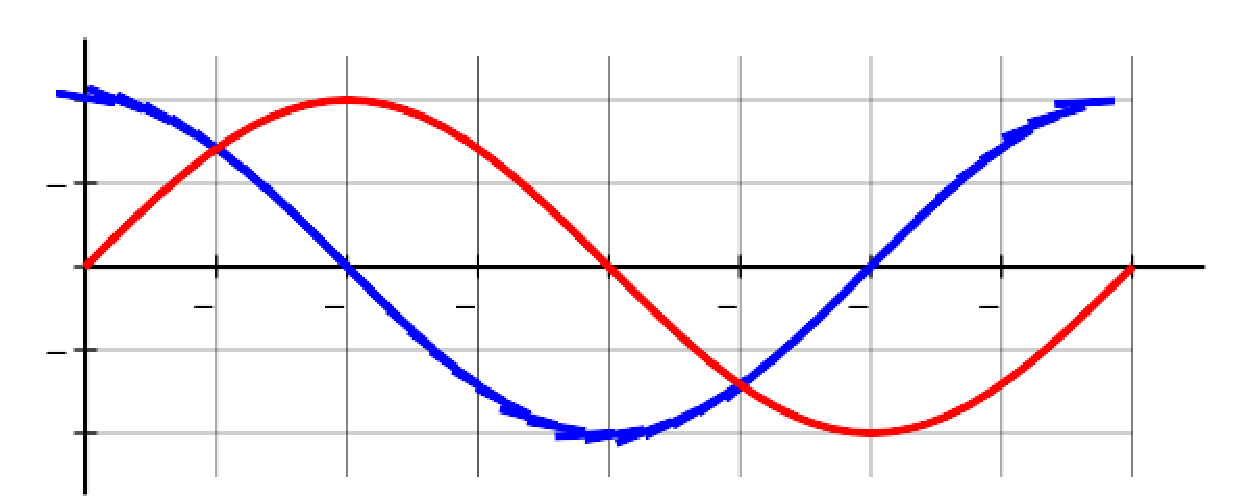
\includegraphics[width=6cm]{\lyxdot \lyxdot /MAIT1/Funktionen/Sine_cosine_one_period} & 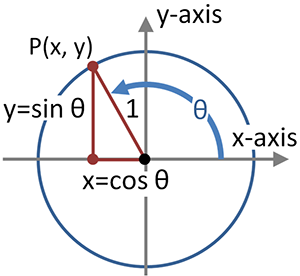
\includegraphics[width=5cm]{\lyxdot \lyxdot /MAIT1/Funktionen/trigfun}\tabularnewline
\end{tabular}
\end{quote}

\subsection*{Polynome}
\begin{quote}
Ein Polynom n-ter Ordnung: $p(x)=a_{n}x^{n}+...+a_{2}x^{2}+a_{1}x+a_{0,}x\in R,a_{n}\neq0$
\end{quote}
Eigenschaften:
\begin{itemize}
\item Differenzen und Summen von Polynomen sind wieder Polynome.
\item Produkte von Polynomen sind wieder Polynome. Bsp: $p(2)\times p(3)=p(5)$
\item Die Division von Polynomen ergiebt wieder ein Polynom und ev. einen
Rest.
\end{itemize}
Beispiel für Polynomdivision:
\begin{verse}
\begin{tabular}{cccccc}
$2x$$^{3}$ & $+5x$$^{2}$ & $+1x$ & $\div(x-5)$ & $=$ & $2x^{2}-5x$ Rest $-24x$\tabularnewline
\hline 
$-2x^{3}$ & $-10x^{2}$ &  & $2x^{2}\times(x-5)$ & $=$ & $2x^{3}-10x^{2}$\tabularnewline
\cline{1-2} 
$0$ & $-5x^{2}$ & $+1x$ & $-5x\times(x-5)$ & $=$ & $-5x^{2}+25x$\tabularnewline
\cline{2-3} 
 & $-(-5x^{2})$ & $-25x$ &  &  & \tabularnewline
\cline{2-3} 
 & $0$ & $-24x$ &  &  & Rest: $-24x$\tabularnewline
\end{tabular}
\end{verse}

\subsubsection*{Hornerschema}

Auswertung einer Funktion an einer bestimmten Stelle.
\begin{verse}
Sei die Funktion $F(x)=x^{3}-3x^{2}-10x+24=(x-2)(x^{2}-x-12)$
\end{verse}
Diese an $x=2$ ausgewertet:
\begin{verse}
\begin{tabular}{ccccc}
\hline 
\multicolumn{1}{|c}{x=2} & $x^{3}$ & $-3x^{2}$ & $-10x$ & \multicolumn{1}{c|}{$24$}\tabularnewline
\hline 
 & 1 & -3 & -10 & 24\tabularnewline
 &  & 2 & -2 & -24\tabularnewline
\hline 
 & 1 & -1 & -12 & 0\tabularnewline
\hline 
Rest: & $x^{2}$ & $-x$ & $-12$ & \tabularnewline
\end{tabular}
\end{verse}
Hier wurde die Nullstelle $x=2$ abgespalten.


\subsection*{Begriffe der Funktionen}


\subsubsection*{Extrema}

$f'(x)=0\, dann\, f''(x_{0})<0\rightarrow Max,\: f''(x_{0})>0\rightarrow Min$


\subsubsection*{Wendestelle}

$f''(x)=0\: dann\: f'''(x_{0})!=0$


\subsubsection*{Ganz-Rationale Funktion}

Eine Ganz-Rationale Funktion lässt sich so schreiben: $f(x)=a_{n}x^{n}+...+a_{2}x^{2}+a_{1}x+a_{0}$


\subsubsection*{Gebrochen-Rationale Funktion}

Eine Gebrochen-Rationale Funktion: $f(x)=\frac{a_{n}x^{n}+...+a_{2}x^{2}+a_{1}x+a_{0}}{b_{n}x^{n}+...+b_{2}x^{2}+b_{1}x+b_{0}}=\frac{p(m)}{p(n)}$,
wobei der Grad der Polynome nicht gleich sein muss.


\subsubsection*{Definitionslücken}

Sie sind Stellen, an denen die Funktion nicht definiert ist. Z.B.:
Nenner der gleich 0 ist. Man unterscheidet 2 Arten von Definitionslücken:
\begin{itemize}
\item Polstellen: Nach dem vollständigen Kürzen, besteht immernoch die Nullstelle
des Nenners.
\item hebbare Definitionslücken: Nach vollständigem Kürzen verschwindet
die Nullstelle des Nenners.
\item Stopfen der Def. Lücke: Wert der hebbaren Lücke in den gekürzten Bruch
einsetzen. 
\end{itemize}
Wichtig: Kommt eine Polstelle mehrmals vor: $(x-a)^{n}$, so ist dies
eine n-fache Polstelle. Ist die Vielfachheit gerade, so findet kein
Vorzeichenwechsel statt.


\subsubsection*{Nullstellen}

Man kann die Nullstellen bestimmen, indem man:
\begin{itemize}
\item bei einer ``Ganz-Rationalen Funktion'' diese gleich NULL setzt.
\item bei einer ``Gebrochen-Rationalen Funktion'' den Zähler gleich NULL
setzt.
\end{itemize}

\subsubsection*{Asymptoten}

Sind Geraden, denen sich eine Kurve beliebig nahe annähert. (Limes!)
Wir unterscheiden 2 Arten:
\begin{itemize}
\item bei Polstellen (nicht hebb. Deflücke): Die Kurve einer gebrochen-rationalen
Funktion schmiegt sich der Gerade bei x=Polstelle an. Es bildet sich
eine senkrechte Asymptote.
\item für grosse x: $f(x)=\frac{g(x)}{h(x)}$ im Falle:

\begin{itemize}
\item $grad(g)<grad(h)$: x-Achse als wagrechte Asymptote
\item $grad(g)=grad(h)$: Gerade mit der Gleichung: $f(x)=\frac{g(x)}{h(x)}$
\item $grad(g)=1+grad(h)$: schiefe Asymptote, durch Polynomdivision
\end{itemize}
\end{itemize}
Man beachte beim Zeichnen die Vielfachheit der Polstelle:
\begin{itemize}
\item Gerade Anzahl: Vorzeichenwechsel
\item Ungerade Anzahl: Kein Vorzeichenwechsel
\end{itemize}
\begin{tabular}{|c|c|}
\hline 
Gerade & Ungerade\tabularnewline
\hline 
$\frac{x^{2}-1}{(x+1)^{2}}$ & $\frac{x^{2}-1}{(x+1)^{3}}$\tabularnewline
\hline 
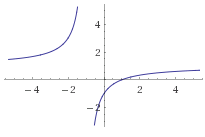
\includegraphics{\lyxdot \lyxdot /MAIT1/Funktionen/vrzw} & 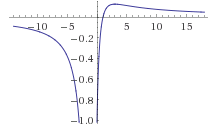
\includegraphics{\lyxdot \lyxdot /MAIT1/Funktionen/kvrzw}\tabularnewline
\hline 
\end{tabular}


\subsubsection*{Beispiele:}
\begin{verse}
\begin{tabular}{|c|c|c|}
\hline 
Funktion & Definitionslücke & Nullstelle\tabularnewline
\hline 
\hline 
$f(x)=\frac{(x+2)^{2}}{(x+4)^{3}x^{2}}$ & P:-4(x3), 0(x2), H: keine & N:-2(x2)\tabularnewline
\hline 
\end{tabular}
\end{verse}


Betrachten wir die Funktion: $f(x)=\frac{2x^{2}+x^{2}+x}{1-x^{2}}$

Nullstelle: $x=0$

Definitionslücken: $x=$1 (Polstelle, 1fach), $x=-1$ (Polstelle,
1fach)

Asymptoten: $x=1$, $x=-1$, $x=-2x-1$ (durch Poly.division)


\section*{Sätze}
\begin{itemize}
\item $sin(\alpha+\beta)=sin(\alpha)\cdot cos(\beta)+cos(\alpha)\cdot sin(\beta)$
\item $sin(\alpha-\beta)=sin(\alpha)\cdot cos(\beta)-cos(\alpha)\cdot sin(\beta)$
\item $cos(\alpha+\beta)=cos(\alpha)\cdot cos(\beta)+sin(\alpha)\cdot sin(\beta)$
\item $sin(\alpha-\beta)=cos(\alpha)\cdot cos(\beta)-sin(\alpha)\cdot sin(\beta)$
\end{itemize}

\section*{Logarithmusfunktion}

Rechenregeln:
\begin{verse}
\begin{tabular}{|c|}
\hline 
$log_{a}(u\cdot v)=log_{a}(u)+log_{a}(v)$\tabularnewline
\hline 
$log_{a}(\frac{u}{v})=log_{a}(u)-log_{a}(v)$\tabularnewline
\hline 
$log_{a}(u^{k})=k\cdot log_{a}(u)$\tabularnewline
\hline 
$log_{a}(\sqrt[n]{u})=\frac{1}{n}\cdot log_{a}(u)$\tabularnewline
\hline 
\end{tabular}
\end{verse}
Allgemein:
\begin{verse}
\begin{tabular}{|c|}
\hline 
$y=a^{x}\Rightarrow ln(y)=x\cdot ln(a)\Rightarrow x=\frac{ln(y)}{ln(a)}$\tabularnewline
\hline 
\end{tabular}

\begin{tabular}{|c|}
\hline 
$y=a^{x}\Rightarrow log_{a}(y)=x\cdot log_{a}(a)\Rightarrow x=log_{a}(y)$ \tabularnewline
\hline 
\end{tabular}
\end{verse}
Umkehrfunktion:
\begin{verse}
\begin{tabular}{|c|}
\hline 
$y=log_{a}(x)$\tabularnewline
\hline 
\end{tabular}
\end{verse}
Basiswechsel:
\begin{verse}
\begin{tabular}{|c|}
\hline 
$log_{a}(x)=\frac{log_{10}(x)}{log_{10}(a)}=\frac{ln(x)}{ln(a)}$\tabularnewline
\hline 
\end{tabular}
\end{verse}
Umformungsbeispiele:
\begin{verse}
\begin{tabular}{|l|l|l|}
\hline 
$log_{10}(x)=-4.0404$ & $\Rightarrow$ & $x=10^{-4.0404}=\frac{1}{10^{4.0404}}$\tabularnewline
\hline 
$ln(x)=-9.0907$ & $\Rightarrow$ & $x=e^{-9.0907}=\frac{1}{e^{9.0907}}$\tabularnewline
\hline 
$log_{3}(x)=5$ & $\Rightarrow$ & $x=3^{5}=243$\tabularnewline
\hline 
\end{tabular}\end{verse}

